\chapter{Ensamblado de Placas de Circuito Impreso}
\section{Introducción}
Es la operación mediante la cual se sitúan y sueldan en la PCI todos los componentes electrónicos que conformen el diseño. El ensamblado se realiza en máquinas automatizadas que aseguran la fiabilidad del proceso y reducen el tiempo de ensamblado. Este proceso es diferente según el encapsulado del componente. Se distinguen tres casos: 
\begin{itemize}
    \item Ensamblado de componentes tradicionales (through-hole)
    \item Ensamblado de componentes SMT (montaje superficial)
    \item Ensamblado manual de componentes que no se pueden montar automáticamente
\end{itemize}

El resultado final es la PCI montada.

\section{Inserción de componentes through-hole}
La inserción de componentes through-hole (TH) es la más compleja debido a la gran diversidad de tipos de encapsulados y de tamaño de componentes. Requiere de máquinas especializadas para cada tipo de encapsulado. El proceso requiere la manipulación del componente, conformado de las patillas, inserción en la PCI y cortado de patillas. La tecnología diferencia los componentes through-hole en los siguientes grupos:
\begin{itemize}
    \item Componentes de encapsulado axial
    \item Componentes de encapsulado radial
    \item Componentes de encapsulado DIP (Dual In Line)
    \item Otros (potenciómetros, conectores, pulsadores, displays, bobinas, transformadores, sensores, etc...)
\end{itemize}

\textbf{Componentes de encapsulado axial.} Las patillas están en el mismo eje que el cuerpo del componente.

\textbf{Componentes de encapsulado radial.} Las patillas son paralelas y perpendiculares al cuerpo del componente.

\subsection{Inserción de componentes axiales}
Requiere una maquinaria específica para el conformado de las patillas, doblado y cortado. La unidad de inserción consta de dos lados simétricos, cada uno de los cuales consta de una pieza de guiado, un conjunto de barra y bloque de corte, y dos piezas - interna y externa - que dan la forma adecuada a las patillas de inserción. Cuando la cabeza de inserción baja, el cortador se mueve hacia dentro, cortando y remachando las patillas en un ángulo ajustable de 0º a 45º relativo al plano de la placa.

Se pueden montar de forma horizontal ó vertical. Es necesario mantener una separación entre el componente y la PCI, para evitar el contacto directo, transferencia de calor de la PCI al componente (y viceversa) y facilitar la aireación del mismo. El conformado de las patillas ha de cumplir con unos requisitos de forma, longitudes, distancia de doblado al cuerpo, etc...Algunos doblados requieren conformados especiales.

\subsection{Inserción de componentes radiales}
La cabeza de inserción radial consta de una mandíbula de inserción que coloca el componente en el circuito impreso. Una vez colocado éste, la pieda de empuje ejerce la presión adecuada sobre el componente para insertarlo correctamente. Debido a que la mandíbula se retira cuando se ejerce la presión de inserción, formando un ángulo de 45º, el layout de inserción de la placa y la propia secuencia de inserción deben diseñarse para asegurarse que no se dañe ningún otro componente ya insertado con este movimiento.

La unidad de corte y remache toma las patillas del componente que sobresalen de la palca y, tras asegurar la disposición uniforme de las mismas, las corta al tamaño adecuado y remacha, asegurando el fijado del componente a la placa.

\subsection{Inserción de componentes DIP}
El encapsulado DIP es típico de los circuitos integrados y zócales. Se usa el mismo principio de guiado que los componentes axiales. La verificación de componentes es una opción disponible en muchas máquinas de inserción DIP. Esta verificación elimina la posibilidad de insertar componentes defectuosos en la máquina o de insertarlos en una posición que no es la adecuada.

Los componentes DIPs se suministran a la máquina de inserción en tubos de plástico llamados DIPs sticks (de material antiestático). Para la inserción se usan unos dedos de inserción, que se colocan aadecuadamente en su posición de partida a unos 15 mm sobre la placa y después bajan el componente correctamente. Existen dos tipos de unidades de corte y remache que doblan las patillas hacia dentro o hacia fuera.


\section{Inserción de componentes SMD - SMT}
Los componentes de montaje superfucial (SMD) (Surface Mount Device) ó de tecnología SMT (Surface Mount Technology) requieren una maquinaria específica. Los encapsulados son más pequeños y están más estandarizados. Esta tecnología aplica a todo tipo de componentes: pasivos, semiconductores y electromecánicos. Permite una mayor velocidad de manejo de las máquinas de posicionamiento de los componentes en la PCI (máquinas de Pick and Place).

Se diferencia respecto a las anteriores en que no existe seguridad de fijación mecánica en la etapa de ensamblado. Se requiere algún tipo de adhesivo que temporalmente mantenga al componente en la posición en que se colocó, hasta que se consiga su fijación definitiva en el proceso de soldadura. El adhesivo temporal puede ser:
\begin{itemize}
    \item Pasta de soldadura depositada en los lugares donde se deberá realizar la posterior soldadura del componente.
    \item Adhesivo para la fijación de los componentes que, tras la soldadura del mismo, será eliminado de diversas maneras.
\end{itemize}

Se utilizan las máquinas de pick and place. Se realiza en tres pasos: 
\begin{enumerate}
    \item Recogida del componente (pick)
    \item Centrado
    \item Posicionado del mismo (place)
\end{enumerate}

El centrado es realizado por medios mecánicos o con la ayuda de visión artificial. La máquina de recogida-posicionado consta de una cabeza que puede girar el componente, en incrementos tan grandes como 90º o tan precisos como 0,01º. La cabeza o huso ejerce una presión de posicionado variable, lo cual permitirá al SMD penetrar en la pasta de soldadura o pegamento con una fuerza controlada.

El mecanismo de centrado se encarga de situar correctamente en función de sus patillas. La visión artificial puede proporcionar asistencia a la acción de centrado. La cámara localiza los lugares donde situar los componentes en la placa relativos a unas marcas de referencia (fisuciales). Los algoritmos de control determinan los movimientos de traslación y rotación necesarios para realizar un posicionado preciso lo más rápido posibles.

La calidad requerida en el posicionado afectará al coste, velocidad y complejidad de la máquina de ensamblado SMT. Se especifican distintos niveles de calidad en el posicionado en función del componente.

\begin{itemize}
    \item Grupo A. Componentes que se deben posicionar con una tolerancia de 0,203 mm a 0.381 mm, dependiendo del tamaño del terminal, tamaño del pad, y de las tolerancias de pad y máquina. Las máquinas de posicionado más simples, de recogida, centrado mecánico y rotaciones en saltos de 90º, son útiles para el montado de estos componentes.
    \item Grupo B. Con menos de 44 terminales requieren un posicionado de calidad moderada.
    \item Grupo C. Componentes que exigen un posicionado de precisión. Estos componentes, con muchos puntos de contacto y terminales cercanos, requieren de visión artificial para su ubicación correcta. La visión se empleará tanto para detectar las marcas en el substrato como para localizar y orientar los terminales de contracto. Los grandes componentes de este grupo necesitan ubicarse con una precisión de hasta 0.051 mm o menos. Debido a la precisión en el montado, la máquina de posicionado deberá incluir la posibilidad de rotación precisa del componente para evitar cortocircuitos o malos contactos.
\end{itemize}

\subsection{Ensamblado mixto SMD - TH}
Algunas aplicaciones requieren montar componentes electrónicos tanto de tipo thorugh-hole (TH) como SMD.

Ensamblado tipo (a): sólo SMD. Se montan componentes SMD en una sola cara de la placa (cara top). Se utiliza para substratos cerámicos o circuitos híbridos.

Ensamblado tipo (b): es la forma más simple de tecnología mixta. Se colocan los componentes TH en la cara superior de la placa (cara top) y SMD sólo en la cara inferior (cara bottom).

Ensamblado tipo (c): se montan componentes TH y SMD en la cara superior (top) y SMD solo, en la capa inferior (bottom). Permite tanto SMT como TH en la misma placa, con la complicación de permitir SMDs en ambas caras de la placa. El mezclar tres procesos distintos hace que este último 

\begin{figure}
    \centering
    \begin{subfigure}[c]{0.3 \textwidth}
        \centering
        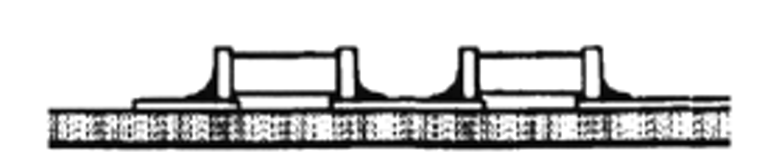
\includegraphics[width = \textwidth]{Imagenes/Ensamblado PCI - Mixto A.png}
        \caption{SMD cara top}
    \end{subfigure}
    \hfill
    \begin{subfigure}[c]{0.3 \textwidth}
        \centering
        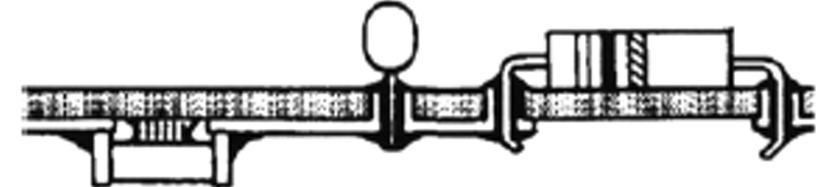
\includegraphics[width = \textwidth]{Imagenes/Encamblado PCI - Mixto B.png}
        \caption{TH cara top y SMD cara bottom}
    \end{subfigure}
    \hfill
    \begin{subfigure}[c]{0.3 \textwidth}
        \centering
        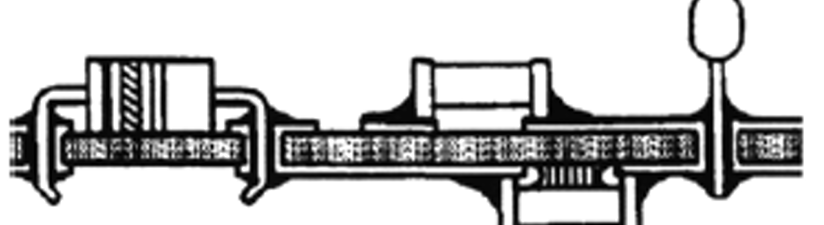
\includegraphics[width = \textwidth]{Imagenes/Ensamblado PCI - Mixto C.png}
        \caption{TH y SMD cara top y SMD cara bottom }
    \end{subfigure}
    \caption{Ensamblado mixto}
\end{figure}

\subsection{Ensamblado manual}

Algunos componentes, por su tamaño y configuración no se pueden montar en máquinas de ensamblado automático. Esto aplica a conectores, interruptores, pulsadores, transformadores, resistencias de potencia de gran tamaño, etc... En este caso, se ha de recurrir al ensamblado manual.

\section{Proceso de soldadura}
La soldadura es el proceso metalúrgico que aplica un metal derretido en la superficie de dos metales a unir, para, después de solidificarse, formar la unión. A la temperatura a la que se lleva a cabo este proceso, el estado físico del material base es sólido y los fluidos o gases de soldadura serán vapor o líquido. Los metales a ser soldados no llegarán nunca a licuarse, y la unión se forma en la interfaz de los dos metales. Aunque el metal base no llegue a licuarse existirá un mezclado de metales en la interfaz, si el metal base es soluble en la aleación de soldadura.

Una soldadura debe cumplir dos funciones:
\begin{enumerate}
    \item Fijar mecánicamente el componente a la PCI
    \item Proporcionar la continuidad eléctrica necesaria entre el componente y las pistas de la PCI.
\end{enumerate}

\section{Inspección del proceso de montaje}